% ============================================================================
% gtfs-ingest -- What changed since the dedupe and MiBici work (Oct-Nov 2026)
%
% Compile from presentations/ (figures are read from ../docs/figures/):
%     latexmk -pdf changes_since_dedupe.tex
%
% Only standard packages: beamer, tikz, listings, lmodern, xcolor, graphicx,
% tabularx. Regenerate the charts first with:
%     python docs/figures/make_figures.py --run outputs/out_mibici_v12 \
%         --before outputs/out_mibici_v9
% Numbers: outputs/out_mibici_v12 and the change logs of each issue (v2 ... v12).
% ============================================================================
\documentclass[aspectratio=169,10pt]{beamer}

\usepackage[utf8]{inputenc}
\usepackage[T1]{fontenc}
\usepackage{lmodern}
\usepackage{microtype}
% keep "--" as two hyphens in code (CLI flags)
\DisableLigatures[-]{encoding = T1, family = tt*}
\usepackage{graphicx}
\usepackage{tabularx}
\usepackage{listings}
\usepackage{tikz}
\usetikzlibrary{positioning, arrows.meta, calc, shapes.geometric, fit, backgrounds}

\graphicspath{{../docs/figures/}}

% ---------------------------------------------------------------------------
% Palette -- identical to the chart palette in docs/figures/make_figures.py,
% so the embedded charts sit seamlessly on the slides.
% ---------------------------------------------------------------------------
\definecolor{cSurface}{HTML}{FCFCFB}
\definecolor{cInk}{HTML}{0B0B0B}
\definecolor{cInkTwo}{HTML}{52514E}
\definecolor{cMuted}{HTML}{898781}
\definecolor{cGrid}{HTML}{E1E0D9}
\definecolor{cBase}{HTML}{C3C2B7}
\definecolor{cContext}{HTML}{D6D5CE}
\definecolor{cCode}{HTML}{F1F0EC}
\definecolor{cBlue}{HTML}{2A78D6}
\definecolor{cOrange}{HTML}{EB6834}
\definecolor{cAqua}{HTML}{1BAF7A}
\definecolor{cYellow}{HTML}{EDA100}
\definecolor{cViolet}{HTML}{4A3AA7}
\definecolor{cRampLight}{HTML}{86B6EF}
\definecolor{cRampDark}{HTML}{0D366B}
% one hue per phase
\colorlet{cPOne}{cBlue}
\colorlet{cPTwo}{cAqua}
\colorlet{cPThree}{cOrange}
\colorlet{cPFour}{cViolet}
\definecolor{cRed}{HTML}{C8322B}
% toy model: one colour per route
\colorlet{cLone}{cRampDark}
\colorlet{cLtwo}{cRampLight}
\colorlet{cRten}{cOrange}
\colorlet{cRtwenty}{cYellow}

% ---------------------------------------------------------------------------
% Beamer look: quiet, ink-on-surface, one accent per phase
% ---------------------------------------------------------------------------
\usetheme{default}
\setbeamertemplate{navigation symbols}{}
\setbeamercolor{background canvas}{bg=cSurface}
\setbeamercolor{normal text}{fg=cInk}
\setbeamercolor{structure}{fg=cBlue}
\setbeamercolor{frametitle}{fg=cInk,bg=cSurface}
\setbeamercolor{title}{fg=cInk}
\setbeamercolor{subtitle}{fg=cInkTwo}
\setbeamercolor{item}{fg=cBlue}
\setbeamercolor{block title}{fg=cInk,bg=cGrid}
\setbeamercolor{block body}{fg=cInk,bg=cCode}
\setbeamercolor{block title alerted}{fg=white,bg=cOrange}
\setbeamercolor{block body alerted}{fg=cInk,bg=cOrange!8}
\setbeamercolor{block title example}{fg=white,bg=cAqua}
\setbeamercolor{block body example}{fg=cInk,bg=cAqua!8}
\setbeamerfont{frametitle}{series=\bfseries,size=\Large}
\setbeamerfont{title}{series=\bfseries,size=\LARGE}
\setbeamertemplate{itemize items}{\raisebox{0.15ex}{\tikz\fill[cBlue] (0,0) circle (0.45ex);}}
\setbeamertemplate{itemize subitem}{\raisebox{0.2ex}{\tikz\fill[cMuted] (0,0) circle (0.35ex);}}
\setbeamertemplate{blocks}[rounded][shadow=false]

\setbeamertemplate{frametitle}{%
  \vskip0.25cm%
  \usebeamerfont{frametitle}\usebeamercolor[fg]{frametitle}\insertframetitle%
  \ifx\insertframesubtitle\empty\else%
    \par\vskip2pt{\normalsize\color{cInkTwo}\mdseries\insertframesubtitle}%
  \fi%
  \vskip0.1cm%
}
\setbeamertemplate{footline}{%
  \hbox to \paperwidth{%
    \hskip0.6cm{\tiny\color{cMuted}gtfs-ingest \,$\cdot$\, What changed%
      \ifx\insertsection\empty\else\,$\cdot$\, \insertsection\fi}%
    \hfill{\tiny\color{cMuted}\insertframenumber\,/\,\inserttotalframenumber}\hskip0.6cm}%
  \vskip0.3cm}

% ---------------------------------------------------------------------------
% Helpers
% ---------------------------------------------------------------------------
\newcommand{\code}[1]{\texttt{\detokenize{#1}}}
\newcommand{\muted}[1]{{\color{cInkTwo}#1}}
\newcommand{\step}[2]{% phase colour, step number -> small coloured badge
  {\setlength{\fboxsep}{2pt}\colorbox{#1}{\scriptsize\bfseries\color{white}STEP #2}}\hspace{0.4em}}

\lstdefinestyle{algo}{
  basicstyle=\ttfamily\scriptsize\color{cInk},
  backgroundcolor=\color{cCode},
  frame=none, framesep=0pt, xleftmargin=6pt, xrightmargin=6pt,
  aboveskip=4pt, belowskip=4pt,
  columns=fullflexible, keepspaces=true, showstringspaces=false,
  commentstyle=\color{cMuted}\itshape,
  keywordstyle=\color{cBlue}\bfseries,
  morekeywords={for,each,if,else,in,emit,drop,sort,by,group,and,or,not,return,while},
  morecomment=[l]{\#},
}
\lstdefinestyle{sql}{
  style=algo, language=SQL, morecomment=[l]{--},
  morekeywords={LATERAL,ST_DWithin,ST_Distance,ST_Transform,ST_MakePoint,ST_SetSRID,
    ST_Buffer,ST_ConvexHull,ST_Collect,ST_Intersects,COALESCE,NULLIF,RETURNING},
}

\tikzset{
  box/.style={draw=#1, fill=#1!9, rounded corners=3pt, align=center, font=\scriptsize,
              inner sep=4pt, text=cInk, line width=0.7pt},
  box/.default=cInkTwo,
  arr/.style={-{Stealth[length=2.2mm,width=1.8mm]}, line width=0.8pt, color=cInkTwo},
  darr/.style={arr, dashed},
  db/.style={cylinder, shape border rotate=90, aspect=0.22, draw=cInkTwo, fill=cContext!45,
             font=\scriptsize, align=center, minimum width=1.9cm, minimum height=1.0cm,
             line width=0.7pt, text=cInk},
  dec/.style={diamond, aspect=2.4, draw=#1, fill=#1!7, font=\tiny, align=center,
              inner sep=0.5pt, text=cInk, line width=0.7pt},
  dec/.default=cInkTwo,
  lbl/.style={font=\tiny, text=cInkTwo},
  yes/.style={font=\tiny\bfseries, text=cAqua!70!black, fill=cSurface, inner sep=1pt},
  no/.style={font=\tiny\bfseries, text=cOrange!80!black, fill=cSurface, inner sep=1pt},
  stop/.style={circle, fill=#1, draw=cSurface, line width=1pt, inner sep=2.6pt},
  stop/.default=cInkTwo,
  st/.style={box=#1, rounded corners=8pt, text width=2.2cm, minimum height=0.8cm},
  nd/.style={circle, draw=#1, fill=#1!12, line width=0.8pt, minimum size=1.15cm, font=\scriptsize\bfseries},
  tbl/.style={draw=#1, fill=cSurface, line width=0.8pt, rounded corners=3pt, anchor=north,
              text width=3.5cm, align=left, font=\tiny\ttfamily, inner sep=4pt},
  head/.style={fill=#1, text=white, font=\scriptsize\bfseries, rounded corners=3pt, anchor=south,
               minimum width=3.5cm+8pt, inner sep=3pt},
}

\newcommand{\cmark}{{\color{cAqua}\ensuremath{\checkmark}}}
\newcommand{\xmark}{{\color{cMuted}\ensuremath{\times}}}

% Toy model (schematic positions, not to scale; real distances are labelled)
\tikzset{
  stRail/.style={circle, fill=cBlue, draw=cSurface, line width=0.8pt, minimum size=8pt, inner sep=0pt},
  stBus/.style={rectangle, fill=cOrange, draw=cSurface, line width=0.8pt, minimum size=7.5pt, inner sep=0pt},
  stBike/.style={diamond, fill=cAqua, draw=cSurface, line width=0.8pt, minimum size=9.5pt, inner sep=0pt},
  unlinked/.style={fill=cSurface, draw=#1, line width=1.2pt},
  etq/.style={font=\scriptsize\bfseries, text=cInk, inner sep=1.5pt},
  tmin/.style={font=\tiny, fill=cSurface, inner sep=0.8pt, text=cInk},
  dist/.style={font=\tiny\itshape, text=cInkTwo, fill=cSurface, inner sep=0.8pt},
  ride/.style={-{Stealth[length=2.2mm,width=1.9mm]}, line width=1.4pt, color=#1},
  routeline/.style={line width=2.6pt, color=#1, opacity=0.3, line cap=round},
  walkarc/.style={densely dashed, line width=1.1pt, color=cInkTwo},
  samest/.style={double=cSurface, double distance=1.3pt, line width=0.7pt, color=cViolet},
  pathhl/.style={line width=6pt, color=cAqua, opacity=0.28, line cap=round, line join=round},
}
\newcommand{\toyCoords}{%
  \coordinate (A1) at (60,320);  \coordinate (A2) at (250,320);
  \coordinate (A3) at (480,320); \coordinate (A4) at (720,320);
  \coordinate (A5) at (800,390); \coordinate (A6) at (800,570);
  \coordinate (B1) at (300,60);  \coordinate (B2) at (300,265);
  \coordinate (B3) at (300,570); \coordinate (B4) at (500,570);
  \coordinate (B5) at (690,570);
  \coordinate (M1) at (60,430);  \coordinate (M2) at (560,110);}
\newcommand{\toyLines}{%
  \draw[routeline=cLone] (A1) -- (A4);
  \draw[routeline=cLtwo] (A5) -- (A6);
  \draw[routeline=cRten] (B1) -- (B3);
  \draw[routeline=cRtwenty] (B3) -- (B5);}
\newcommand{\toyStops}{%
  \node[stRail, label={[etq]below left:A1}] (nA1) at (A1) {};
  \node[stRail, label={[etq]above left:A2}] (nA2) at (A2) {};
  \node[stRail, label={[etq]above:A3}] (nA3) at (A3) {};
  \node[stRail, label={[etq]above:A4}] (nA4) at (A4) {};
  \node[stRail, label={[etq]right:A5}] (nA5) at (A5) {};
  \node[stRail, label={[etq]right:A6}] (nA6) at (A6) {};
  \node[stBus, label={[etq]right:B1}] (nB1) at (B1) {};
  \node[stBus, label={[etq]below right:B2}] (nB2) at (B2) {};
  \node[stBus, label={[etq]above:B3}] (nB3) at (B3) {};
  \node[stBus, label={[etq]above:B4}] (nB4) at (B4) {};
  \node[stBus, label={[etq]above:B5}] (nB5) at (B5) {};
  \node[stBike, label={[etq]left:M1}] (nM1) at (M1) {};
  \node[stBike, label={[etq]below:M2}] (nM2) at (M2) {};}
\newcommand{\toyRides}{%
  \draw[ride=cLone] (nA1) -- node[tmin, below] {2.0} (nA2);
  \draw[ride=cLone] (nA2) -- node[tmin, below, pos=0.3] {2.0} (nA3);
  \draw[ride=cLone] (nA3) -- node[tmin, below] {2.0} (nA4);
  \draw[ride=cLtwo] (nA5) -- node[tmin, left] {1.5} (nA6);
  \draw[ride=cRten] (nB1) -- node[tmin, left] {3.0} (nB2);
  \draw[ride=cRten] (nB2) -- node[tmin, left, pos=0.6] {3.5} (nB3);
  \draw[ride=cRtwenty] (nB3) -- node[tmin, below] {3.0} (nB4);
  \draw[ride=cRtwenty] (nB4) -- node[tmin, below] {2.5} (nB5);}
\newcommand{\toyDistances}{%
  \node[dist, right] at ($(A1)!0.5!(M1)$) {20 m};
  \node[dist] at (215,270) {0 m};
  \node[dist, below right] at ($(A4)!0.5!(A5)$) {28 m};
  \node[dist, below] at ($(A6)!0.5!(B5)+(0,-10)$) {71 m};}
\newcommand{\toyStopLegend}{%
  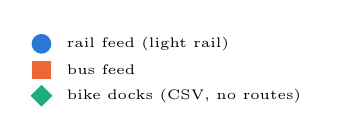
\begin{tikzpicture}[font=\tiny, x=1cm, y=1cm]
    \node[stRail] at (0,0) {};      \node[anchor=west] at (0.2,0) {rail feed (light rail)};
    \node[stBus] at (0,-0.33) {};   \node[anchor=west] at (0.2,-0.33) {bus feed};
    \node[stBike] at (0,-0.66) {};  \node[anchor=west] at (0.2,-0.66) {bike docks (CSV, no routes)};
  \end{tikzpicture}}
\newcommand{\toyArcLegend}{%
  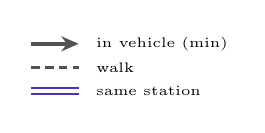
\begin{tikzpicture}[font=\tiny, x=1cm, y=1cm]
    \draw[ride=cInkTwo] (0,0) -- (0.6,0);   \node[anchor=west] at (0.7,0) {in vehicle (min)};
    \draw[walkarc] (0,-0.3) -- (0.6,-0.3);  \node[anchor=west] at (0.7,-0.3) {walk};
    \draw[samest] (0,-0.6) -- (0.6,-0.6);   \node[anchor=west] at (0.7,-0.6) {same station};
  \end{tikzpicture}}
\newcommand{\toyRouteLegend}{%
  
\begin{tikzpicture}[font=\tiny, x=1cm, y=1cm]
    \draw[line width=2pt, cLone] (0,0) -- (0.45,0);        \node[anchor=west] at (0.5,0) {L1};
    \draw[line width=2pt, cLtwo] (1.0,0) -- (1.45,0);      \node[anchor=west] at (1.5,0) {L2};
    \draw[line width=2pt, cRten] (2.0,0) -- (2.45,0);      \node[anchor=west] at (2.5,0) {R10};
    \draw[line width=2pt, cRtwenty] (3.1,0) -- (3.55,0);   \node[anchor=west] at (3.6,0) {R20};
  \end{tikzpicture}}

% Big number tile: value, label, accent
\newcommand{\stat}[3]{%
  \tikz\node[draw=#3, fill=#3!8, line width=0.8pt, rounded corners=4pt, minimum width=3.3cm,
             minimum height=1.5cm, align=center, inner sep=3pt]
    {{\LARGE\bfseries\color{cInk}#1}\\[3pt]{\scriptsize\color{cInkTwo}#2}};}

% Section divider: phase name, colour, subtitle, step list
\newcommand{\divider}[4]{%
  \begin{frame}[plain]
    \begin{tikzpicture}[remember picture, overlay]
      \fill[#2] (current page.north west) rectangle ([xshift=0.45cm]current page.south west);
      \node[anchor=west, font=\fontsize{30}{34}\selectfont\bfseries, text=cInk]
        at ([xshift=1.4cm, yshift=1.2cm]current page.west) {#1};
      \node[anchor=west, font=\large, text=cInkTwo]
        at ([xshift=1.42cm, yshift=0.15cm]current page.west) {#3};
      \node[anchor=north west, font=\small, text=cInk, align=left, text width=12cm]
        at ([xshift=1.42cm, yshift=-0.5cm]current page.west) {#4};
    \end{tikzpicture}
  \end{frame}}

% Severity badge for the validation table
\newcommand{\sevbadge}[2]{\tikz[baseline=(s.base)]\node[fill=#1,text=white,rounded corners=1.5pt,
  inner sep=1.6pt,font=\tiny\bfseries](s){\strut #2};}
\newcommand{\sevE}{\sevbadge{cOrange}{ERROR}}
\newcommand{\sevW}{\sevbadge{cYellow}{WARN}}
\newcommand{\sevI}{\sevbadge{cMuted}{INFO}}
% Data-model table: name, title, colour, x, y, body
\newcommand{\tb}[6]{%
  \node[head=#3] (#1h) at (#4,#5) {#2};
  \node[tbl=#3] (#1) at (#4,#5) {#6};}

\title{gtfs-ingest: What Changed Since Dedupe and MiBici}
\subtitle{From the within-feed dedupe and the MiBici stops CSV to routing-ready data ---
  Guadalajara Metropolitan Area}
\author{Víctor Rodríguez}
\date{\today}

\newcommand{\pill}[2]{{\setlength{\fboxsep}{2.5pt}\colorbox{#1}{\scriptsize\bfseries\color{white}#2}}}
\newcommand{\badge}[2]{\tikz[baseline=(s.base)]\node[fill=#1,text=white,rounded corners=1.5pt,
  inner sep=1.6pt,font=\tiny\bfseries](s){\strut #2};}
\newcommand{\done}{\badge{cAqua}{FIXED}}
\newcommand{\partly}{\badge{cYellow}{BY DESIGN}}
\newcommand{\still}{\badge{cOrange}{OPEN}}

\begin{document}

% ============================================================================
\begin{frame}[plain]
  \begin{tikzpicture}[remember picture, overlay]
    \fill[cAqua]   ([yshift=-0.35cm]current page.north west) rectangle ++(4cm,0.35cm);
    \fill[cBlue]   ([xshift=4cm,yshift=-0.35cm]current page.north west) rectangle ++(4cm,0.35cm);
    \fill[cOrange] ([xshift=8cm,yshift=-0.35cm]current page.north west) rectangle ++(4cm,0.35cm);
    \fill[cViolet] ([xshift=12cm,yshift=-0.35cm]current page.north west) rectangle ++(4cm,0.35cm);
  \end{tikzpicture}
  \vskip1.6cm
  {\usebeamerfont{title}\usebeamercolor[fg]{title}\inserttitle\par}
  \vskip0.35cm
  {\large\color{cInkTwo}\insertsubtitle\par}
  \vskip1.2cm
  {\normalsize\insertauthor\par}
  {\small\color{cMuted}\insertdate\par}
  \vfill
  {\scriptsize\color{cMuted}Before: the run \code{out_mibici_v2} (October 2026, within-feed radius 50\,m, MiBici with
   walk arcs) $\cdot$ after: \code{outputs/out_mibici_v12} $\cdot$ both with 2 GTFS feeds + MiBici, OSM network walk,
   300\,m proximity}
\end{frame}

% ============================================================================
\begin{frame}{From v2 to v12}
  \framesubtitle{Every step was measured on a full database run before moving on}
  \centering
  \resizebox{\textwidth}{!}{%
  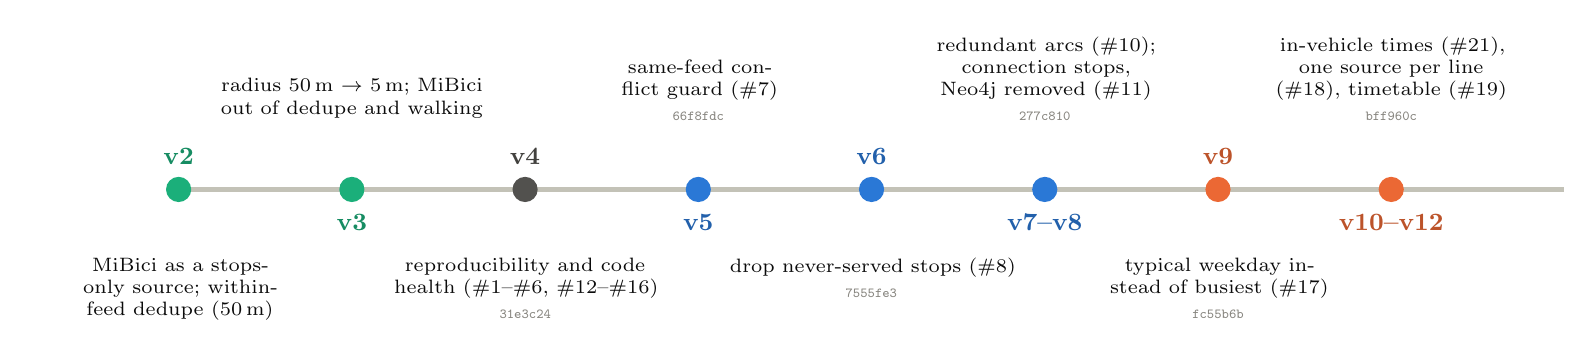
\begin{tikzpicture}[x=1cm,y=1cm]
    \draw[cBase, line width=2pt] (0,0) -- (17.6,0);
    % labels alternate below and above the line so neighbours never overlap
    \foreach \x/\run/\col/\what/\commit/\side in {
      0.0/v2/cAqua/{MiBici as a stops-only source; within-feed dedupe (50\,m)}//-1,
      2.2/v3/cAqua/{radius 50\,m $\rightarrow$ 5\,m; MiBici out of dedupe and walking}//1,
      4.4/v4/cInkTwo/{reproducibility and code health (\#1--\#6, \#12--\#16)}/31e3c24/-1,
      6.6/v5/cBlue/{same-feed conflict guard (\#7)}/66f8fdc/1,
      8.8/v6/cBlue/{drop never-served stops (\#8)}/7555fe3/-1,
      11.0/v7--v8/cBlue/{redundant arcs (\#10); connection stops, Neo4j removed (\#11)}/277c810/1,
      13.2/v9/cOrange/{typical weekday instead of busiest (\#17)}/fc55b6b/-1,
      15.4/v10--v12/cOrange/{in-vehicle times (\#21), one source per line (\#18), timetable (\#19)}/bff960c/1}
    {
      \fill[\col] (\x,0) circle (0.16);
      \node[font=\small\bfseries, text=\col!80!black] at (\x,-0.42*\side) {\run};
      \node[font=\scriptsize, text=cInk, align=center, text width=3.6cm,
            anchor={\ifnum\side>0 south\else north\fi}] at (\x,0.75*\side) {\what\\[1pt]{\tiny\ttfamily\color{cMuted}\commit}};
    }
  \end{tikzpicture}}
  \vskip0.5cm
  \small
  \begin{columns}[T]
    \column{0.32\textwidth}\centering\stat{8,877 $\rightarrow$ 10,203}{physical stations}{cAqua}
    \column{0.32\textwidth}\centering\stat{50 $\rightarrow$ 1}{station-network components}{cBlue}
    \column{0.32\textwidth}\centering\stat{0 $\rightarrow$ 3.29\,M}{timetable connections}{cOrange}
  \end{columns}
\end{frame}

% ============================================================================
\begin{frame}{Before and after}
  \framesubtitle{\code{out_mibici_v2} (or the first run that measured it) against \code{out_mibici_v12}}
  \scriptsize
  \renewcommand{\arraystretch}{1.18}
  \begin{tabularx}{\textwidth}{@{}>{\raggedright\arraybackslash}X r r >{\raggedright\arraybackslash}p{5.2cm}@{}}
    \hline
    \textbf{Measure} & \textbf{before} & \textbf{v12} & \textbf{Why} \\ \hline
    stop records in the outputs & 14,349 & 12,768 & 1,581 never-served mdb stops left out (\#8) \\
    physical stations & 8,877 & \textbf{10,203} & opposite platforms no longer merge \\
    within-feed alias pairs & 2,697 (median 28.9\,m) & 247 ($\le$ 4.6\,m) & radius 50\,m $\rightarrow$ 5\,m \\
    widest station & 103\,m & 7.5\,m & same-feed conflict guard (\#7) \\
    walk arcs touching a MiBici dock & 5,756 & 0 & docks are unlinked nodes \\
    station-network weak components & 50 & \textbf{1} & never-served stops formed the pieces \\
    one-way-reachable stops & 86 (v3) & 9 & typical weekday, not a holiday (\#17) \\
    service dates & 2020-01-01, 2024-01-01 & 2021-05-04, 2024-06-27 & both old dates were holidays \\
    routes in the routing network & 274 & 249 & 38 lines published twice dropped (\#18) \\
    0-minute in-vehicle arcs & 31 (v8) & 1 & aliases under one \code{stop_sequence} (\#21) \\
    \code{MT_L3} peak headway & 230--330\,s (v9) & 420\,s & directions relabelled (\#21) \\
    timetable & --- & 3,290,920 connections & \code{connections.csv.gz} (\#19) \\
    two runs, same files & no & \textbf{yes} & sorting, tie-breaks, manifest (\#1--\#5) \\ \hline
  \end{tabularx}
\end{frame}

% ============================================================================
\section{MiBici}
\divider{MiBici as a stops-only source}{cAqua}{484 bike-share docks: geometry, no schedule}{%
  One predicate drives every branch \,$\cdot$\, where the docks show up \,$\cdot$\, out of dedupe and walking}

% ============================================================================
\begin{frame}{One predicate drives every branch}
  \framesubtitle{\code{FeedSource.is_stops_only} --- an explicitly named \code{.csv} is a feed that contributes stops only}
  \begin{columns}[T]
    \column{0.5\textwidth}
    \small
    \begin{itemize}
      \item \textbf{Discovery} tags a named \code{.csv} as \code{kind="csv"}; a folder scan never picks up CSVs ---
            a previous run's \code{near_stations.csv} would re-enter as a second network
      \item \code{feed_id} from the stem: \code{mibici.csv} $\rightarrow$ \code{mibici}
      \item The CSV reader resolves headers by alias (\code{Latitud}, \code{lat}, \code{LATITUDE}\ldots), any delimiter,
            UTF-8 with BOM, UTF-16 or cp1252
      \item Phase 2 handles it \textbf{before} any service-date logic: no calendar, early return, status \code{stops_only}
    \end{itemize}
    \column{0.47\textwidth}
    \scriptsize
    \renewcommand{\arraystretch}{1.25}
    \begin{tabularx}{\linewidth}{@{}l c >{\raggedright\arraybackslash}X@{}}
      \hline
      \textbf{Output} & \textbf{Docks?} & \textbf{How} \\ \hline
      stops, PostGIS, GeoPackage & \cmark & every stop output \\
      proximity pairs & \cmark & \code{geographic_feed_ids} \\
      \code{near_stations.csv} & \cmark & own row; neighbour with line \code{-} \\
      station network & node & \textbf{no arcs} (unlinked) \\
      dedupe & \xmark & excluded from both rules \\
      route graph, headways & \xmark & no routes or trips \\
      timetable & \xmark & no trips \\ \hline
    \end{tabularx}
    \vskip0.2cm
    \begin{alertblock}{A bug dry runs could not show}
      \scriptsize The PostGIS proximity query filtered on \emph{analysed} feeds only, so docks got no neighbours in full
      runs. Dry runs used a local join that ignored the list. Now stops-only feeds are in it.
    \end{alertblock}
  \end{columns}
\end{frame}

% ============================================================================
\begin{frame}{MiBici out of dedupe and out of walking}
  \framesubtitle{Two risks closed by rule, not by luck}
  \begin{columns}[T]
    \column{0.48\textwidth}
    \pill{cBlue}{DEDUPE}\par\vskip4pt
    \small A dock named after a corner, within 30\,m of a bus stop with the same name, could merge with it as
    ``the same station''. It never happened only because MiBici names start with \code{(GDL-001)}.
    \textbf{Now stops-only sources are excluded from both dedupe rules.}
    \column{0.48\textwidth}
    \pill{cAqua}{WALKING}\par\vskip4pt
    \centering
    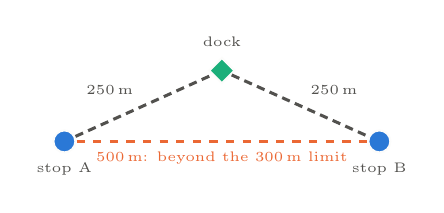
\begin{tikzpicture}[x=1cm,y=1cm]
      \node[stRail] (a) at (0,0) {}; \node[lbl, below] at (a.south) {stop A};
      \node[stBike] (d) at (2,0.9) {}; \node[lbl, above] at (d.north) {dock};
      \node[stRail] (b) at (4,0) {}; \node[lbl, below] at (b.south) {stop B};
      \draw[walkarc] (a) -- node[lbl, above left] {250\,m} (d);
      \draw[walkarc] (d) -- node[lbl, above right] {250\,m} (b);
      \draw[dashed, cOrange, line width=0.8pt] (a) -- node[lbl, below, text=cOrange] {500\,m: beyond the 300\,m limit} (b);
    \end{tikzpicture}
    \raggedright
    \vskip2pt
    \small Docks were stepping stones between distant stops. \textbf{Now they have no walk arcs.}
  \end{columns}
  \vskip0.4cm
  \begin{columns}[T]
    \column{0.32\textwidth}\centering\stat{0}{docks merged with stops}{cAqua}
    \column{0.32\textwidth}\centering\stat{5,756 $\rightarrow$ 0}{walk arcs touching a dock}{cAqua}
    \column{0.32\textwidth}\centering\stat{1,901 $\rightarrow$ 0}{shortcuts that existed only via docks}{cAqua}
  \end{columns}
\end{frame}

% ============================================================================
\section{Stations}
\divider{What counts as a station}{cBlue}{From 8,877 to 10,203 physical stations}{%
  50\,m $\rightarrow$ 5\,m \,$\cdot$\, the same-feed conflict guard (\#7) \,$\cdot$\, never-served stops (\#8)}

% ============================================================================
\begin{frame}{Why the within-feed radius went from 50\,m to 5\,m}
  \framesubtitle{A duplicate record sits at 0\,m; the other direction's platform is across the street}
  \begin{columns}[c]
    \column{0.55\textwidth}
    \centering
    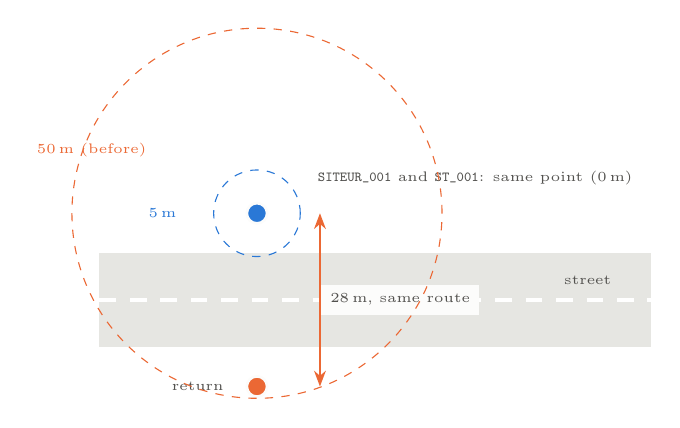
\begin{tikzpicture}[x=1cm,y=1cm]
      \fill[cContext!60] (-0.5,0.9) rectangle (6.5,2.1);
      \draw[white, line width=1.2pt, dash pattern=on 6pt off 5pt] (-0.5,1.5) -- (6.5,1.5);
      \node[lbl] at (5.7,1.75) {street};
      \node[stop=cBlue] (n) at (1.5,2.6) {};
      \node[stop=cOrange] (s) at (1.5,0.4) {};
      \node[lbl, anchor=west] at (2.15,3.05) {\code{SITEUR_001} and \code{ST_001}: same point (0\,m)};
      \node[lbl, anchor=east] at (1.2,0.4) {return};
      \draw[{Stealth[length=2mm]}-{Stealth[length=2mm]}, cOrange, line width=0.8pt] (2.3,2.6) -- node[lbl, right, fill=cSurface] {28\,m, same route} (2.3,0.4);
      \draw[dashed, cBlue] (1.5,2.6) circle (0.55);
      \node[lbl, text=cBlue] at (0.3,2.6) {5\,m};
      \draw[dashed, cOrange] (1.5,2.6) circle (2.35);
      \node[lbl, text=cOrange] at (-0.6,3.4) {50\,m (before)};
    \end{tikzpicture}
    \column{0.43\textwidth}
    \small
    \begin{itemize}
      \item At \textbf{50\,m} the rule joined the outbound and the return platform: same route, 20--40\,m apart.
      \item Two platforms became ``one station'', which gave a \textbf{free U-turn} when routing (0-minute alias arc).
      \item At \textbf{5\,m} only records really listed twice are joined.
    \end{itemize}
    \vskip4pt
    \begin{exampleblock}{Measured}
      \scriptsize Within-feed pairs: 2,697 (median 28.9\,m) $\rightarrow$ \textbf{247}, all between 0 and 4.6\,m.
    \end{exampleblock}
  \end{columns}
\end{frame}

% ============================================================================
\begin{frame}{Chaining, and the same-feed conflict guard (\#7)}
  \framesubtitle{Cross-feed pairs could still chain two opposite platforms of one feed through the other feed}
  \begin{columns}[c]
    \column{0.47\textwidth}
    \centering
    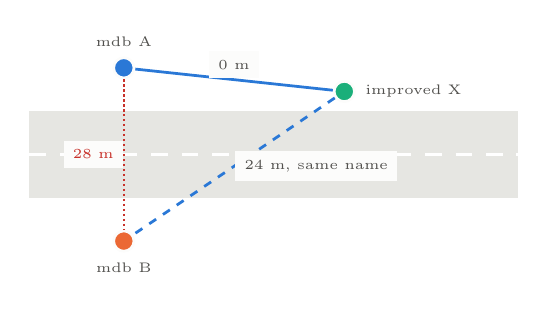
\begin{tikzpicture}[x=1cm,y=1cm]
      \fill[cContext!60] (-0.6,0.95) rectangle (5.6,2.05);
      \draw[white, line width=1.2pt, dash pattern=on 6pt off 5pt] (-0.6,1.5) -- (5.6,1.5);
      \node[stop=cBlue, label={[lbl]above:{mdb A}}] (a) at (0.6,2.6) {};
      \node[stop=cOrange, label={[lbl]below:{mdb B}}] (b) at (0.6,0.4) {};
      \node[stop=cAqua, label={[lbl]right:{improved X}}] (x) at (3.4,2.3) {};
      \draw[cBlue, line width=1pt] (a) -- node[lbl, above, fill=cSurface] {0 m} (x);
      \draw[cBlue, line width=1pt, dashed] (x) -- node[lbl, right, fill=cSurface] {24 m, same name} (b);
      \draw[cRed, line width=0.8pt, densely dotted] (a) -- node[lbl, left, text=cRed, fill=cSurface] {28 m} (b);
    \end{tikzpicture}
    \vskip0.2cm
    \scriptsize Greedy union, closest pairs first: reject a pair that would put two stops of one feed more than 5\,m
    apart in one group. Rejected pairs stay neighbours.
    \column{0.5\textwidth}
    \scriptsize
    \renewcommand{\arraystretch}{1.25}
    \begin{tabular}{@{}l r r@{}}
      \hline
      & \textbf{v4} & \textbf{v5 (\#7)} \\ \hline
      physical stations & 10,533 & 11,054 \\
      groups with far same-feed stops ($>$ 15\,m) & 283 & \textbf{0} \\
      widest station & 103\,m & 7.5\,m \\
      pairs rejected & --- & 1,077 \\
      route graph edges & 9,112 & 9,112 \\ \hline
    \end{tabular}
    \vskip0.2cm
    \muted{The rejected pairs' conflicts are 5.2\,m or more apart (median 20.5\,m): opposite platforms. A simulation
    before coding predicted exactly these numbers.}
  \end{columns}
\end{frame}

% ============================================================================
\begin{frame}{Never-served stops (\#8)}
  \framesubtitle{1,581 mdb stops are in \code{stops.txt} but in no \code{stop_times} row}
  \begin{columns}[c]
    \column{0.5\textwidth}
    \small
    \begin{itemize}
      \item 738 duplicate a served stop of the other feed; 843 are listed with no trip at all.
      \item 111 of them formed the \textbf{49 small pieces} of the station network: nothing could reach them.
      \item Now left out of every output by default (\code{--no-drop-unserved-stops} keeps them); still loaded into
            PostGIS, which keeps the full inventory.
    \end{itemize}
    \column{0.47\textwidth}
    \scriptsize
    \renewcommand{\arraystretch}{1.25}
    \begin{tabular}{@{}l r r@{}}
      \hline
      & \textbf{v5 (keep)} & \textbf{v6 (drop)} \\ \hline
      stop records in outputs & 14,349 & 12,768 \\
      physical stations & 11,054 & \textbf{10,203} \\
      weak components (transit) & 50 & \textbf{1} \\
      walk arcs & 186,150 & 144,572 \\
      pairs rejected by \#7 & 1,077 & 772 \\
      interchanges (multimodal) & 2,708 (71) & 2,565 (73) \\ \hline
    \end{tabular}
  \end{columns}
  \vskip0.3cm
  \centering
  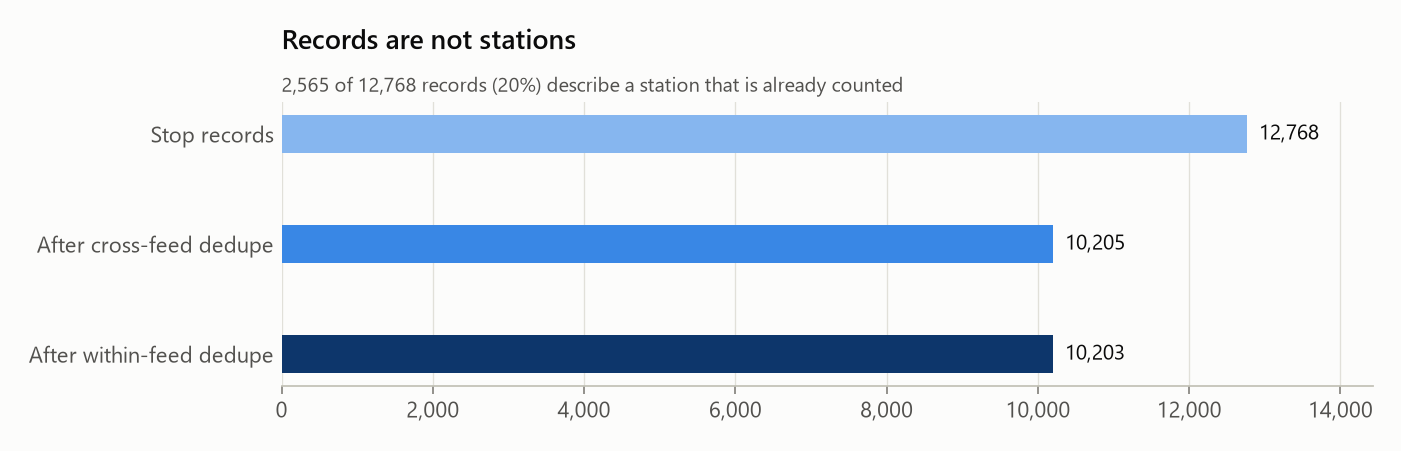
\includegraphics[width=0.62\textwidth]{r1_records_to_stations.png}
\end{frame}

% ============================================================================
\begin{frame}{Dedupe today}
  \begin{columns}[c]
    \column{0.6\textwidth}
    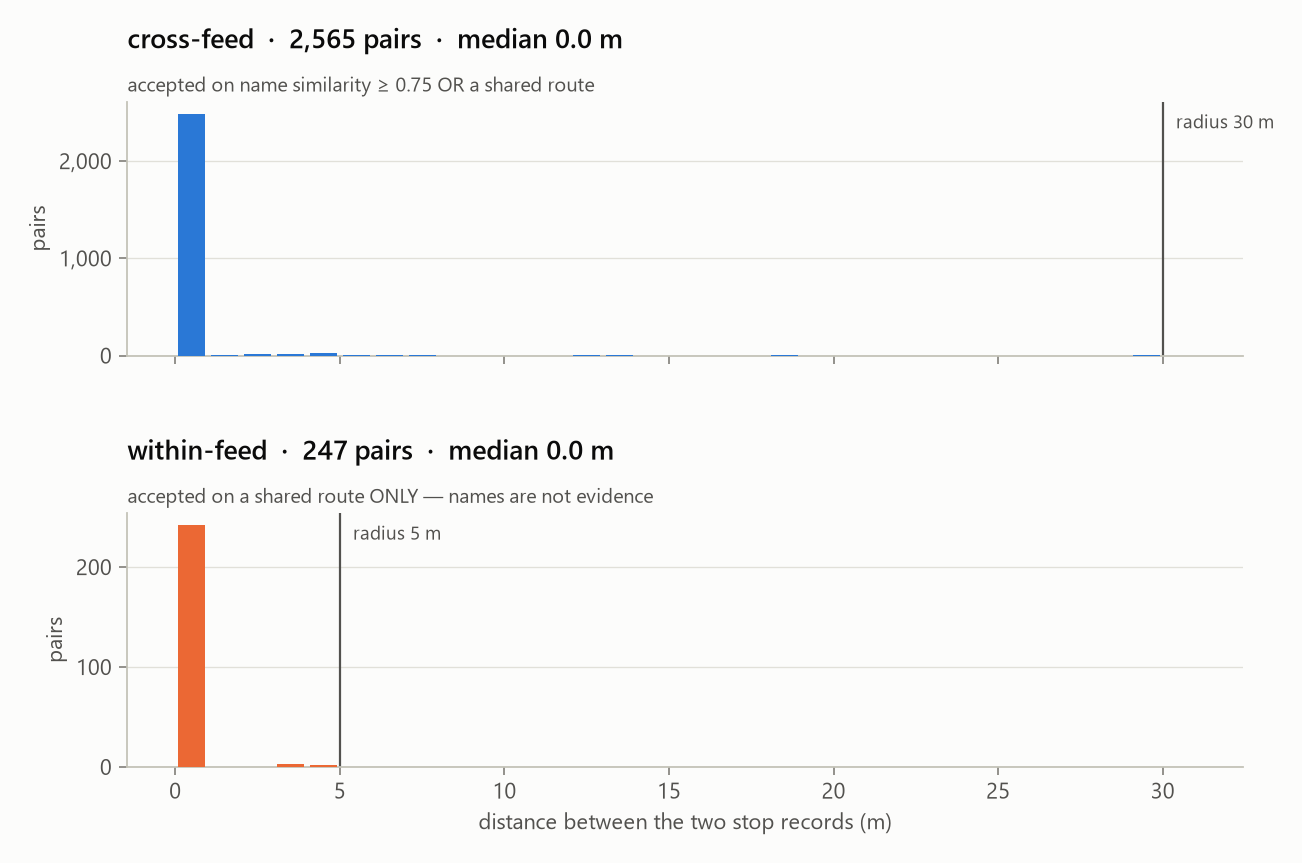
\includegraphics[width=\linewidth]{r2_dedupe_distances.png}
    \column{0.38\textwidth}
    \small
    \begin{itemize}
      \item \textbf{2,565 cross-feed pairs}, median 0.0\,m: the feeds share a stop inventory.
      \item \textbf{247 within-feed pairs}, all $\le$ 4.6\,m: one station recorded twice.
      \item \textbf{1,604 groups}, widest 7.5\,m, median span 0\,m.
      \item MiBici: never merged.
    \end{itemize}
    \vskip0.2cm
    \begin{block}{A station is a platform group}
      \scriptsize Opposite platforms are separate stations joined by walk links --- the right model for routing.
    \end{block}
  \end{columns}
\end{frame}

% ============================================================================
\section{Network and outputs}
\divider{Network and outputs}{cBlue}{Make the outputs cleaner and easier to use}{%
  Redundant arcs (\#10) \,$\cdot$\, where routes connect (\#11) \,$\cdot$\, Neo4j removed \,$\cdot$\, a geography index}

% ============================================================================
\begin{frame}{Redundant arcs (\#10)}
  \framesubtitle{Many walk arcs never change a shortest time --- reported always, pruned on request}
  \begin{columns}[c]
    \column{0.45\textwidth}
    \centering
    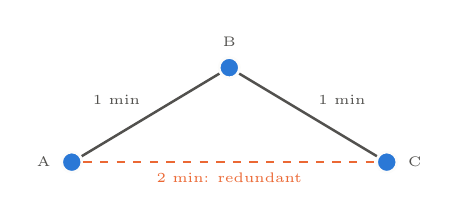
\begin{tikzpicture}[x=1cm,y=1cm]
      \node[stop=cBlue, label={[lbl]left:A}] (a) at (0,0) {};
      \node[stop=cBlue, label={[lbl]above:B}] (b) at (2,1.2) {};
      \node[stop=cBlue, label={[lbl]right:C}] (c) at (4,0) {};
      \draw[cInkTwo, line width=0.9pt] (a) -- node[lbl, above left] {1 min} (b);
      \draw[cInkTwo, line width=0.9pt] (b) -- node[lbl, above right] {1 min} (c);
      \draw[cOrange, line width=0.9pt, dashed] (a) -- node[lbl, below, text=cOrange] {2 min: redundant} (c);
    \end{tikzpicture}
    \vskip0.2cm
    \scriptsize Removed longest first, only if the remaining walking network still links the two stops within the
    same minutes; alias pairs keep a spanning tree per station.
    \column{0.52\textwidth}
    \scriptsize
    \renewcommand{\arraystretch}{1.3}
    \begin{tabular}{@{}l r r@{}}
      \hline
      & \textbf{default} & \textbf{\code{--prune-station-network}} \\ \hline
      walk pairs & 72,286 & 29,729 \\
      same\_station pairs & 2,812 & 2,565 \\
      weak components & 1 & 1 \\ \hline
    \end{tabular}
    \vskip0.25cm
    \begin{exampleblock}{Verified}
      \scriptsize Dijkstra from 300 random stops on both GraphMLs: identical \code{time_min} distances for all
      3,683,106 reachable pairs.
    \end{exampleblock}
  \end{columns}
\end{frame}

% ============================================================================
\begin{frame}{Where routes connect (\#11), and Neo4j removed}
  \begin{columns}[T]
    \column{0.52\textwidth}
    \pill{cBlue}{ROUTE CONNECTION CSVs}\par\vskip4pt
    \scriptsize
    \renewcommand{\arraystretch}{1.25}
    \begin{tabularx}{\linewidth}{@{}l >{\raggedright\arraybackslash}X@{}}
      \hline
      \code{route_connections.csv} & one row per route pair = the GraphML edges \\
      \code{route_connection_stops.csv} & \textbf{where}: every route pair and stop pair behind an edge, with type and distance \\
      \code{routes.csv}, \code{route_stops.csv} & decode the uids; \code{duplicate_of} since \#18 \\ \hline
    \end{tabularx}
    \vskip0.2cm
    For every route pair, the strongest type in \code{route_connection_stops.csv} equals the edge's type.
    \column{0.45\textwidth}
    \pill{cInkTwo}{NEO4J EXPORT REMOVED}\par\vskip4pt
    \scriptsize The CSVs replace the graph-database package: the same relations, readable in pandas, R or QGIS, with
    no server. The command, its module, tests and docs were deleted.
    \vskip0.3cm
    \pill{cAqua}{GEOGRAPHY INDEX}\par\vskip4pt
    \scriptsize A GiST index on \code{geom::geography} for the proximity query:
    \vskip3pt
    \centering\stat{2\,min 18\,s $\rightarrow$ 2\,s}{proximity query}{cAqua}
    \raggedright
    \vskip3pt
    \muted{\tiny The slow query had dropped a database connection mid-run.}
  \end{columns}
\end{frame}

% ============================================================================
\section{Reproducibility}
\divider{Reproducibility}{cInkTwo}{Two runs, the same files --- and healthier code}{%
  Deterministic ids and order (\#1--\#3) \,$\cdot$\, run manifest (\#4) \,$\cdot$\, golden test (\#5)
  \\[4pt] ruff, packaging, smaller functions, faster ranges (\#12--\#16)}

% ============================================================================
\begin{frame}{Two runs, the same files}
  \begin{columns}[T]
    \column{0.5\textwidth}
    \scriptsize
    \renewcommand{\arraystretch}{1.3}
    \begin{tabularx}{\linewidth}{@{}l >{\raggedright\arraybackslash}X@{}}
      \hline
      \textbf{Issue} & \textbf{Change} \\ \hline
      \#1 IDs & \code{near_stations} \code{ID} numbered by \code{stop_uid}, not by \code{--feeds} order \\
      \#2 ties & every sort is stable (mergesort) with a full tie-break \\
      \#3 SQL & every query has \code{ORDER BY}; nearest-node ties broken by \code{osm_id} \\
      \#4 manifest & \code{run_manifest.json}: input sha256s, git commit, code hash, versions, parameters; no secrets \\
      \#5 golden & a fixed two-feed run byte-compared with committed CSVs \\ \hline
    \end{tabularx}
    \column{0.47\textwidth}
    \begin{exampleblock}{Checked on every full run since}
      \scriptsize v4 = v4b, v5 = v5b, v9 = v9b, v12 = v12b: every CSV, GraphML, GeoPackage layer and
      \code{connections.csv.gz} byte-identical; reports differ only in their timestamp.
    \end{exampleblock}
    \vskip0.2cm
    \begin{alertblock}{An index trap}
      \scriptsize Adding \code{osm_id} straight to the KNN \code{ORDER BY} stopped PostGIS from using the spatial
      index: \code{conflate-osm} ran 23+ minutes instead of seconds. A 5-candidate subquery keeps the index and the
      tie-break.
    \end{alertblock}
  \end{columns}
\end{frame}

% ============================================================================
\begin{frame}{Code health}
  \begin{columns}[T]
    \column{0.5\textwidth}
    \scriptsize
    \renewcommand{\arraystretch}{1.3}
    \begin{tabularx}{\linewidth}{@{}l >{\raggedright\arraybackslash}X@{}}
      \hline
      \#12 packaging & every subpackage in the wheel; CI checks it \\
      \#13 ruff & rules pinned, lint and format blocking in CI \\
      \#14 split & \code{_analyze_feed} and \code{run_analysis} split into small steps \\
      \#15 ranges & days with the same services analysed once: 3\,min 02\,s $\rightarrow$ 1\,min 19\,s \\
      \#16 cleanup & unused tooling and a stray venv removed \\ \hline
    \end{tabularx}
    \vskip0.2cm
    \muted{\scriptsize Formatting was AST-verified: no code or docstring changed.}
    \column{0.47\textwidth}
    \centering
    \stat{303 $\rightarrow$ 347}{tests, incl. live PostGIS}{cInkTwo}
    \vskip0.3cm
    \raggedright
    \begin{itemize}\scriptsize
      \item CLI and config defaults share one constant, guarded by a test
      \item Sphinx \code{-W} and ruff in CI
      \item One default source per flag: \code{--fix-directions}, \code{--route-dedupe}, \code{--min-transfer-s}, \ldots
    \end{itemize}
  \end{columns}
\end{frame}

% ============================================================================
\section{Routing data}
\divider{Routing-ready data}{cOrange}{The inputs a routing benchmark needs}{%
  A typical weekday (\#17) \,$\cdot$\, in-vehicle times (\#21) \,$\cdot$\, one source per line (\#18)
  \,$\cdot$\, the timetable (\#19)}

% ============================================================================
\begin{frame}{A typical weekday, not the busiest day (\#17)}
  \framesubtitle{``Busiest'' was a holiday in both feeds: Sunday service stacked on weekday service}
  \begin{columns}[T]
    \column{0.5\textwidth}
    \small
    \textbf{Rule:} Mon--Fri dates with service that \code{calendar_dates} doesn't touch $\rightarrow$ the most common
    service set $\rightarrow$ the middle Tue--Thu date.
    \vskip0.2cm
    \scriptsize
    \begin{itemize}
      \item \code{--date-rule busiest} keeps the old rule
      \item \code{--feed-service-date F=D} pins one feed
      \item \code{service_dates_note} explains why dates differ
    \end{itemize}
    \column{0.47\textwidth}
    \scriptsize
    \renewcommand{\arraystretch}{1.25}
    \begin{tabular}{@{}l r r@{}}
      \hline
      & \textbf{busiest (v8)} & \textbf{typical (v9)} \\ \hline
      improved date & 2020-01-01 & \textbf{2021-05-04} \\
      mdb date & 2024-01-01 & \textbf{2024-06-27} \\
      mdb trips & 807 & 511 \\
      T16B directions & 1 & 2 \\
      one-way-reachable stops & 55 & 9 \\
      route graph routes & 274 & 287 \\ \hline
    \end{tabular}
  \end{columns}
  \vskip0.3cm
  \begin{alertblock}{Still two years}
    \scriptsize The calendars never overlap (improved 2020--2022, mdb 2024), so each feed keeps its own day. After
    \#18 only two improved routes remain in the routing inputs.
  \end{alertblock}
\end{frame}

% ============================================================================
\begin{frame}{In-vehicle times (\#21)}
  \begin{columns}[c]
    \column{0.55\textwidth}
    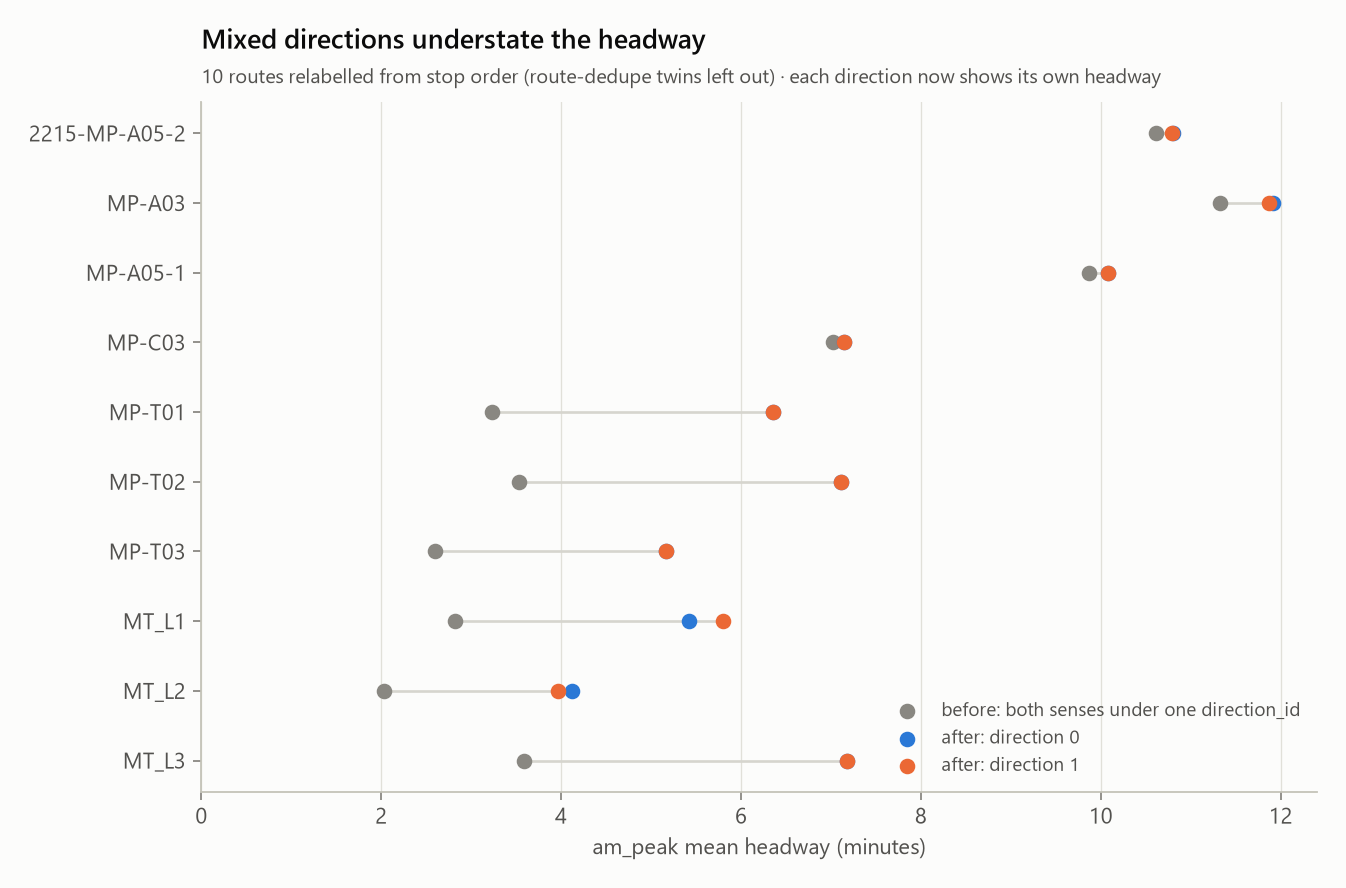
\includegraphics[width=\linewidth]{r12_direction_fix.png}
    \column{0.43\textwidth}
    \scriptsize
    \textbf{Directions:} 19 trips on 19 routes carried both senses under one \code{direction_id}; relabelled from
    stop order. \code{MT_L3} now shows its published 420\,s.
    \vskip0.15cm
    \textbf{Stop order:} mdb \code{MT_L1}/\code{MT_L2} list each station twice under one \code{stop_sequence}; one
    stop kept per sequence. 0-minute arcs 31 $\rightarrow$ 1.
    \vskip0.15cm
    \textbf{Trust:} \code{time_quality} on every arc and connection --- 18 \code{too_fast} ($>$ 80\,km/h), 4
    \code{too_slow} (T16B placeholders at 70\,min), 1 \code{zero}. Times are kept.
    \vskip0.15cm
    \textbf{Explained:} the 484 stops with no travel time are the MiBici docks.
  \end{columns}
\end{frame}

% ============================================================================
\begin{frame}{One source per line (\#18)}
  \begin{columns}[c]
    \column{0.55\textwidth}
    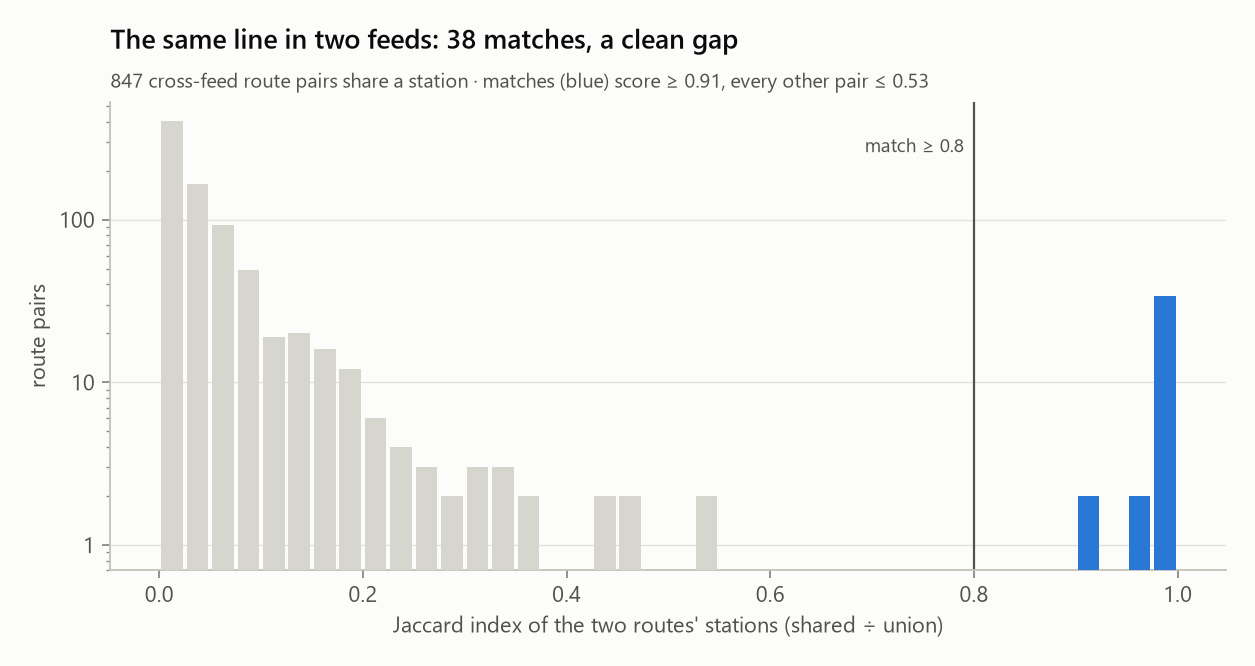
\includegraphics[width=\linewidth]{r11_route_jaccard.png}
    \column{0.43\textwidth}
    \scriptsize
    \begin{itemize}
      \item improved is almost a subset of mdb: 38 of its 40 routes are mdb routes with a \code{2215-} prefix and
            identical departures
      \item Short names can't match lines: \code{L1}--\code{L3} are both Mi Tren and SiTren
      \item Stop sets mapped to stations: matches $\ge$ 0.91, others $\le$ 0.53; the newer feed wins
      \item mdb lists every SiTren trip twice: 8 dropped
    \end{itemize}
    \vskip0.1cm
    \renewcommand{\arraystretch}{1.2}
    \begin{tabular}{@{}l r r@{}}
      \hline
      & \textbf{before} & \textbf{after} \\ \hline
      routes in the graph & 287 & 249 \\
      route links & 10,255 & 7,902 \\
      \code{in_vehicle} arcs & 26,388 & 24,036 \\ \hline
    \end{tabular}
  \end{columns}
\end{frame}

% ============================================================================
\begin{frame}{The timetable (\#19)}
  \begin{columns}[c]
    \column{0.56\textwidth}
    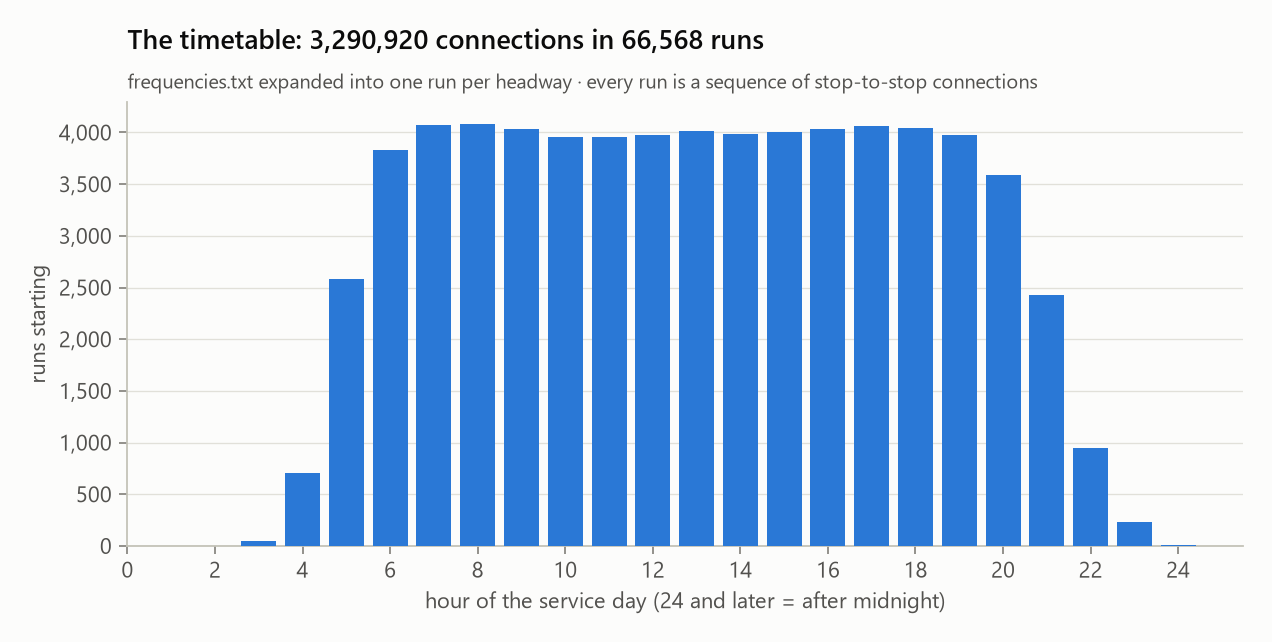
\includegraphics[width=\linewidth]{r13_timetable_by_hour.png}
    \column{0.42\textwidth}
    \scriptsize
    \begin{itemize}
      \item \code{connections.csv.gz}: every vehicle hop of the day, frequencies expanded, sorted by departure
      \item \code{footpaths.csv}: walk links both ways, alias links and a 120\,s change time per stop
      \item 61\,MB compressed: 66,568 runs $\times$ $\approx$49 stops; about 550\,MB as plain CSV
      \item Byte-identical across runs; every arc matches its connections
      \item A CSA scan from 08:00 reaches 99.8--99.9\,\% of the 10,499 served stops
    \end{itemize}
  \end{columns}
\end{frame}

% ============================================================================
\section{Status}
\divider{Status}{cInk}{What the October review found, and where it stands}{%
  Open problems \,$\cdot$\, review findings \,$\cdot$\, next steps}

% ============================================================================
\begin{frame}{The October review, revisited}
  \scriptsize
  \renewcommand{\arraystretch}{1.22}
  \begin{tabularx}{\textwidth}{@{}c >{\raggedright\arraybackslash}p{4.4cm} >{\raggedright\arraybackslash}X@{}}
    \hline
    & \textbf{Problem (Oct 2026)} & \textbf{Now} \\ \hline
    \done & Opposite platforms still joined (283 groups) & conflict guard (\#7): 0 groups, widest station 7.5\,m \\
    \done & Station network not connected (50 pieces) & never-served stops dropped (\#8): 1 component \\
    \done & 86 stops reachable one way only & typical weekday (\#17): 9, all route terminals \\
    \done & Route graph ``fragile'' at T16B (2 bridges) & checked (\#9): the bridges cut off two 3-stop feeders \\
    \done & Many redundant walk arcs & counted on every run, \code{--prune-station-network} (\#10) \\
    \partly & Feeds analysed on different dates & typical weekday each; the calendars never overlap \\
    \partly & Route graph depends on the 300\,m radius & without walking the graph splits where BRT/rail is reached on foot \\
    \done & CLI and config defaults differed & one constant per default, test-guarded \\
    \done & Report omitted the within-feed radius & \code{dedupe_within_feed_distance_m} in the report \\
    \done & Docks could merge with bus stops; docks extended walks & excluded from dedupe; unlinked in the network \\
    \done & Free U-turns through alias arcs & 5\,m rule + conflict guard \\
    \done & \code{ID} depended on \code{--feeds} order & numbered by \code{stop_uid} (\#1) \\ \hline
  \end{tabularx}
\end{frame}

% ============================================================================
\begin{frame}{Next steps}
  \begin{columns}[T]
    \column{0.48\textwidth}
    \pill{cOrange}{ROUTING DATA}\par\vskip4pt
    \scriptsize
    \begin{itemize}
      \item \#20 frequency-based graph: waiting and transfer cost
      \item \#22 access and egress: walk from any point to nearby stops
      \item \#23 a clean merged GTFS for reference engines
    \end{itemize}
    \vskip0.2cm
    \pill{cViolet}{ROUTING BENCHMARK}\par\vskip4pt
    \begin{itemize}
      \item \#24 one interface for every algorithm
      \item \#25 Dijkstra baselines: static, frequency-based, time-dependent
      \item \#26 CSA and RAPTOR on \code{connections.csv.gz}
      \item \#27 query sets, metrics and a \code{benchmark-routing} command
      \item \#28 compare with OpenTripPlanner 2 or r5py
    \end{itemize}
    \column{0.48\textwidth}
    \pill{cInkTwo}{CODE HEALTH}\par\vskip4pt
    \scriptsize
    \begin{itemize}
      \item \#29 figures regenerated from v12 --- done for these decks
      \item \#30 presentation decks and paper numbers
      \item \#31 clean up old runs in \code{outputs/}
    \end{itemize}
    \vskip0.3cm
    \begin{exampleblock}{Ready now}
      \scriptsize A static graph for Dijkstra (\code{station_network.graphml}) and a full-day timetable for CSA and
      RAPTOR (\code{connections.csv.gz} + \code{footpaths.csv}), both reproducible from the same command.
    \end{exampleblock}
  \end{columns}
\end{frame}

\end{document}
